\chapter{Modellbildung}\label{mod}
Um ein System zu verbessern, sind genaue Kenntnisse darüber notwendig. Deshalb ist das Wissen der beteiligten Komponenten zur Energieumwandlung Voraussetzung für die Optimierung. Zur Modellbildung können zwei Arten von Strategien angewendet werden. Entweder kann das Modell auf der Verallgemeinerung von Messdaten durch Mustervergleiche oder auf physikalischen, chemischen Grundgleichungen basieren \cite{Mauracher1996}. Im Folgenden werden wir die Modellbildung anhand von Mustervergleichen einfacher Bauelemente einführen. \\\\

Bevor es zur Vorstellung einfacher Komponenten in einem elektrochemischen System kommt, werden wir elektrotechnische Grundlagen kennenlernen und an einfachem System anwenden. 

\section{Kirchhoffsche Regeln}\label{mod:kirch}
\begin{itemize}
\item Punkte, in denen drei oder mehrere Leitungen zusammentreffen heißen \glqq Knoten\grqq\ oder \glqq Verzweigungspunkte\grqq. Knoten können keine Ladungen speichern. Daher führt das Gesetz der Ladungserhaltung auf die erste kirchhoffsche Regel. In einem Knoten ist die Summe aller zufließenden Ströme gleich der Summe aller abfließenden Ströme.
	  \[
		\sum_n I_n = 0
	  \]
	  Ein Netzwerk mit n Knoten hat n-1 unabhängige Knotengleichungen.
\item Geschlossene Teilkreise eines Netzwerkes heißen \glqq Maschen\grqq. Für Maschen gilt die zweite 				Kirchhoff'sche Regel oder Maschenregel: Beim Durchlaufen einer Masche ist die Summe aller Spannungen null.
\end{itemize}
\cite[S.63]{Kuypers2012B2}
\subsection{Einfaches Modell}
\begin{figure}[ht]
	\centering
	\def\svgwidth{0.9\columnwidth}
	\input{images/einfachesModell.eps_tex}
	\caption{Einfaches Modell: Widerstand mit RC - Glied}
	\label{fig:einfachModell}
\end{figure}
Das in Abbildung \ref{fig:einfachModell} dargestellte Modell hat zwar Bezug zu einer Batterie, bildet aber aus einen Teil der Komponenten einer Batterie ab und soll ausschließlich zur Veranschaulichung der Theorie in \ref{sys} des Eingabe / Ausgabesystems dienen. \\\\
Wenden wir uns den Kirchhoffsche Regeln \ref{mod:kirch} zu. Dann folgt für die Knoten:
\begin{align}
	I = I_1 + I_2
\end{align}
sowie für die Maschen
\begin{align}
	I \cdot R_\Omega + R_{ct} \cdot I_2 - U = 0	\\
	V_{C_{dl}} - R_{ct} \cdot I_2 = 0
\end{align}
Die folgende Zwangsbedingungen grenzen die Freiheitsgrade ein:
\begin{align}
I_1 &= I_{C_{dl}} \\
I_{C_{dl}} &=  C \cdot \frac{d}{dt} V_{C_{dl}}
\end{align}
\begin{bem}
Die zweite Zwangsbedingung gilt aufgrund des elektrischen Verhaltens eines Kondensators im Stromkreis.
\end{bem}
Damit lässt sich nun das System $\mathscr{S}$ eindeutig beschreiben. Einsetzen und Umformungen führen auf folgende Gleichung
\begin{align}
I\cdot (R_{\Omega} + R_{ct}) + C \cdot R_{\Omega} \cdot R_{ct} \frac{d}{dt} I &= U + R_{ct} \cdot C \cdot \frac{d}{dt} U 
\end{align}
Die Gleichung wird nun in die Form eines einfachen Eingabe  / Ausgabe Systems gebracht
\begin{align}
q(\xi):&=(R_{\Omega} + R_{ct})+C \cdot R_{\Omega} \cdot R_{ct} \cdot \xi\\
p(\xi):&=(1+C\cdot R_{ct}\cdot \xi) \\\notag\\
\Rightarrow p(\frac{d}{dt}) \cdot U &= q(\frac{d}{dt})\cdot I
\Leftrightarrow p(\frac{d}{dt}) \cdot U - q(\frac{d}{dt})\cdot I = 0\\
&\begin{bmatrix}
p(\frac{d}{dt}) & -q(\frac{d}{dt})
\end{bmatrix}
\cdot 
\begin{bmatrix}
U \\ 
I
\end{bmatrix}
= 0
\end{align}
und mit Satz \ref{sys:general} kann die Übertragungsfunktion im Signalbereich gefunden werden. 
\begin{align}
H(s)&=p^{-1}(s)\cdot q(s)\\
\Rightarrow H(s) &= R_{\Omega} + \frac{R_{ct}}{1 + C \cdot R_{ct} \cdot s }
\end{align}
Da in diesem Beispiel die Imaginärachse im Konvergenzbereich der Laplace - Transformation liegt, folgt für die Fouriertransformation
\begin{align}
H(i\omega) 		&= R_{\Omega} + \frac{R_{ct}}{1 + C \cdot R_{ct} \cdot i\omega }\\
			 	&= R_{\Omega} + \frac{R_{ct}}{1 + (C \cdot R_{ct} \cdot \omega)^2 } - i \cdot \omega \cdot \frac{C \cdot R_{ct}^2}{1 + (C \cdot R_{ct} \cdot \omega)^2 }\label{gl:Trans}
\end{align}
Mit Satz \ref{sys:faltung} folgt für das einfache Modell das es beschränkt ist, und mit Satz \ref{s:Impuls} in ein Faltungssystem übergeführt werden kann. Somit existiert die Impedanz. Es gilt $Z(\omega) := H(\omega)$.\\
Man betrachte man nun im Folgenden die Gleichung 
\begin{align}
	S(\omega) = Z(\omega) - R_{innen} =  \frac{R_{ct}}{1 + (C \cdot R_{ct} \cdot \omega)^2 } - i \cdot \omega \cdot \frac{C \cdot R_{ct}^2}{1 + (C \cdot R_{ct} \cdot \omega)^2 } \text{.}
\end{align}
Für $S(\omega)$ kann nun nach Satz \ref{sys:titch:rational} ein Zusammenhang zwischen Real - und Imäginarteil herstellen werden. 
\begin{bem}
	In der Praxis wird bei der Hilbert - Transformation der Innenwiderstand abgezogen. Um den Innenwiderstand zu ermitteln muss der Punkt gefunden werden, bei dem es für den Imaginärteil der Impedanz zu einem Vorzeichenwechsel kommt.
\end{bem}

Im Folgenden werden wir wegen des Rechenaufwandes mit komplexen Widerständen rechnen. Dies ist eine äquivalente Darstellung im Frequenzbereich zu den Differentialgleichungen mit konstanten Koeffizienten im Zeitbereich \ref{sys:diff}.
\begin{itemize}\label{mod:rules}
	\item Ohmsches Gesetz:  $U = Z I$ 
	\item Ohmscher Widerstand: 	$Z_R = R$
	\item Induktiver Blindwiderstand: $Z_L = i \omega L$
	\item Kapazitiver Blindwiderstand: $Z_C = \frac{1}{i \omega C}$
	\item Reihenschaltung:  $Z = \sum_{i = 1}^{n} Z_i$
	\item Paralleschaltung: $\frac{1}{Z} = \sum_{i=1}^{n} Z_i$
\end{itemize}\cite[Seite 183]{Kuypers2012B2}

\section{Komponenten eines elektrochemischen Systems}
\subsection{Innenwiderstand}
$R_{innen}$ spiegelt den ohmischen Widerstand der Elektroden, Stromableiter und Elektrolyten wieder. Er liegt je nach Größe und Anwendungsbereich der Zelle im Bereich zwischen $1 m\Omega$ bis zu $100 m\Omega$.
\subsection{RC - Glied}
Das RC - Glied besteht aus einem Widerstand (engl. Resistor) und einem Kondensator (engl. Capacitor) 
und besitzt folgende Impedanz
\begin{align}
	Z(i \omega) = \frac{R}{1+ R i \omega C } = \frac{\frac{1}{C}}{i \omega + \frac{1}{C \cdot R}} \label{mod:rc:gl} \text{, }
\end{align}
außerdem diese Übertragungsfunktion 
\begin{align}
Z(s) = \frac{\frac{1}{C}}{s + \frac{1}{C \cdot R}} \quad \text{, } \Re{s} > - \frac{1}{C \cdot R}\label{mod:RC:trans}
\end{align}
Für den Zeitbereich gilt dann (Tabelle \ref{lt:exp})
\begin{align}
	h(t) =  \frac{1}{C} \exp{- \frac{1}{R C}}  \quad t  > 0 \label{mod:RC:time}
\end{align}
Mit Hilfe von einzelnen oder mehreren RC - Gliedern kann die Doppelsichtkapazität und Durchtrittsreaktion, die sich an den Kontaktflächen zwischen  Elektrolyt und Elektrode ausbilden, abgebildet werden. 

\subsection{Darstellung des Diffusionseffektes}
Das Warburg - Element bildet die Diffusion innerhalb des Elektrolyts nach und macht dementsprechend auch eine Aussage über die kinetische Eigenschaften der Zeile. Wir werden die Warburg - Elemente und die CPE - Elemente nur als Mustervergleich einführen. Physikalische Hintergründe können in \cite{Mauracher1996} oder \cite{MacDonald2005} nachgelesen werden. Im Folgenden werden nun für die Arbeit relevanten Warburg - Elemente und CPE - Elemente genannt.
\subsection{Das Endliche Warburg Element} \label{mod:warburg}
\begin{align}
	Z_{W}(i \omega) = \frac{\tanh{a \sqrt{i \omega}}}{\sqrt{i \omega}}  \label{mod:warburg:gl}
\end{align}
Die Warburg - Impedanz ist weder in $\lint{1}{\mathbb{R}}$ noch in $\lint{2}{\mathbb{R}}$ und es kann nicht mit Hilfe des Satzes von Titchmarsh \ref{ht:titch} ein Bezug von Realteil und Imaginärteil hergestellt werden. Es muss eine andere Möglichkeit gefunden werden. \\
\subsubsection{Approximation des endlichen Warburg Elements}\label{mod:finiteWarburg}
Die folgenden Sätze zeigen, dass das Warburg - Element mit Hilfe von RC - Gliedern approximiert werden kann und somit den Satz von Titchmarsh \ref{ht:titch} erfüllt. \\
Dazu werden wir die Impedanz für eine infinites Warburg - Element durch die Laplace - Transformation von dem Bildbereich in den Signalbereich und approximativ wieder zurück in Bildbereich transformieren. 
\begin{satz}
Sei $s \in \mathbb{C}$, $t \in \mathbb{R}_{\geq 0}$ und $F(s) = \frac{\tanh{a \sqrt{s}}}{\sqrt{s}}$ dann ist die Umkehrfunktion gegeben mit
\begin{align}
	\lt{\frac{\tanh{a \sqrt{s}}}{\sqrt{s}}} = \frac{2}{a} \cdot \sum_{k=1}^{\infty}  \exp{-\frac{\pi^2}{4 a^2} \left( 2 k - 1 \right) t} \label{mod:umkehr}
\end{align}
eine bijektive Abbildung für $\Re{s} > - \frac{\pi^2}{4 a^2}$
\begin{proof}
Sei $f(t):= \sum_{k=1}^{\infty} \frac{2}{a} \cdot \exp{-\frac{\pi^2}{4 a^2} \left( 2 k - 1 \right) t}$. Dann ist $f(t)\in \ltr{-\frac{\pi^2}{4 a^2}}$ (siehe Anhang \ref{a:L_stetig}) und $f(t)$ stetig differenzierbar.\\ 
Des Weiteren wird die Gleichung \ref{mod:warburg:gl} mit $Z(s) =:F(s)$ und dessen Grenzwert von 
\begin{align}
	\lim_{R \rightarrow \infty} \sup_{\abs{s} = R} \abs{F(s)} = \lim_{R \rightarrow \infty} \sup_{\abs{s} = R} \frac{\tanh{a \sqrt{s}}}{\sqrt{s}} = 0
\end{align} betrachtet.
Anwendung des L'Hospital führt zu 
\begin{align}
	\lim_{R \rightarrow \infty} \sup_{\abs{s} = R} \frac{\tanh{a \sqrt{s}}}{\sqrt{s}} = \lim_{R \rightarrow \infty} \sup_{\abs{s} = R} \frac{2 a \sqrt{s}}{2 \cdot \cosh{\sqrt{s}}^2 \sqrt{s}} = 0
\end{align} Somit sind alle Voraussetzungen für die Residuenformel der inversen Laplace - Transformation \ref{lt:res} erfüllt und wir können den Residuensatz \ref{a:res} anwenden. Dazu müssen zuerst alle Singularitäten ermittelt werden.
\begin{description}
\item[Punkt $s=0$] ~\par
	Die Anwendung von L'Hospital liefert sofort 
	\begin{align}
	\lim_{R \rightarrow 0} \sup_{\abs{s} = R} \frac{\tanh{a \sqrt{s}}}{\sqrt{s}} = \lim_{R \rightarrow 0} \sup_{\abs{s} = R} \frac{2 a \sqrt{s}}{2 \cdot \cosh{\sqrt{s}}^2 \sqrt{s}}	 = a \text{, }
	\end{align}
	dass der Punkt $s = s_0$ eine hebbare Polstelle ist, d.h. weder ein Verzweigungspunkt noch eine Singularität.
\item[Punkte $\cosh{\sqrt{s}} = 0$] ~\par
Die Funktion $F(s) = \frac{\tanh{a \sqrt{s}}}{\sqrt{s}} = \frac{\sinh{a \sqrt{s}}}{\sqrt{s} \cdot \cosh{a \sqrt{s}}}$ hat hingegen unendlich viele Polstellen, die durch folgende Gleichung
\begin{align}
	\cosh{a \sqrt{s}} = \frac{\exp{a \sqrt{s}} + \exp{-a \sqrt{s}}}{2} = 0
\end{align}
gegeben sind.
Es werden die Singularitäten folgendermaßen bestimmt:
\begin{align}
	\exp{2 a \sqrt{s}} &= -1 = \exp{\pi i + 2 k \pi i} \quad \text{, mit } k=0, \pm 1, \pm 2\text{, ...} \\
	2 a \sqrt{s} &= (k + \frac{1}{2}) \pi i \Leftrightarrow s = - \frac{\pi}{4 a^2} \left[2 k + 1 \right]
\end{align}
Anzumerken wäre noch, dass diese Singularitäten Pole erster Ordnung darstellen
\end{description}
Daraus lassen sich nun mit Satz \ref{a:respol} die  
Residuen in den Punkten $s_n = -\frac{\pi^2}{4 a^2} \left( 2 k + 1 \right)$ bestimmen
		\begin{align}
			\res{\exp{st}F(s)}{s_n} &=  \lim_{s \rightarrow s_n} (s - s_n) \left\{ \frac{\exp{st} \tanh{a \sqrt{s}} }{\sqrt{s}}  \right\}\\
			&=\lim_{s \rightarrow s_n} (s - s_n) \left\{ \frac{\exp{st} \sinh{a \sqrt{s}} }{\sqrt{s} \cdot \cosh{a \sqrt{s}}}  \right\}\\
			&=\lim_{s \rightarrow s_n} \left\{\frac{s - s_n}{\cosh{a \sqrt{s}}}\right\} \cdot  \lim_{s \rightarrow s_n} \left\{ \frac{\exp{st} \sinh{a \sqrt{s}}}{ \sqrt{s}}\right\}
		\end{align}
		Nun wird der erste Term mit L'Hospital ausgewertet:
		\begin{align}
			&\lim_{s \rightarrow s_n} \left\{ \frac{2 \sqrt{s}}{a  \cdot \sinh{a \sqrt{s}}} \right\} \cdot  \lim_{s \rightarrow s_n} \left\{ \frac{\exp{st} \sinh{a \sqrt{s}}}{ \sqrt{s}}\right\}\\
			&= \frac{2}{a} \cdot \exp{-\frac{\pi^2}{4 a^2} \left( 2 k + 1 \right) t}
		\end{align}
		
Dann folgt insgesamt für unendliche viele Singularitäten und $t > 0$
\begin{align}
	\mathscr{L}^{-1} \left\{\frac{\tanh{a \sqrt{s}}}{\sqrt{s}} \right\} = \frac{2}{a} \cdot \sum_{k=1}^{\infty}  \exp{-\frac{\pi^2}{4 a^2} \left( 2 k - 1 \right) t} =f(t)
\end{align}
Nach Satz \ref{s:expTyp} folgt sofort, dass die Laplacetransformierte existiert, d.h. die Abbildung 
\ref{mod:umkehr} bijektiv für $\Re{s} > -\frac{\pi^2}{4 a^2}$ ist.
\end{proof}
\end{satz}
Ein Vergleich der Umkehrfunktion \ref{mod:umkehr} mit dem Zeitbereich eines RC - Gliedes \ref{mod:RC:time} zeigt, dass sich die Warburg - Impedanz durch eine Reihenschaltung von endlich vielen RC - Gliedern approximieren lässt. Die Impulsantwort $h(t)$ dieser Reihenschaltung hat dann die Form:
\begin{align}
	h(t) &= \sum_{k = 1}^{n} \frac{1}{C_k} \exp{-\frac{t}{R_k C_k}} \quad \text{, mit}\\
	C_k  &= \frac{a}{2}  \\
	R_k 	 &= \frac{8 a}{(2 k - 1)^2 \pi^2} \quad \text{und } t > 0
\end{align}
Mit der Linearität der Laplace - Transformation folgt für die Approximation der Übertragungsfunktion des Warburg - Elements
\begin{align}
	H(s) \approx  \sum_{k = 1}^{n} \frac{\frac{1}{C_k}}{s + \frac{1}{R_k \cdot C_k}} \quad \text{, mit } \Re{s} \geq 0 
\end{align}
Da die Null in Konvergenzbereich enthalten ist, folgt unmittelbar für die approximierte Impedanz
\begin{align}
	Z(i \omega) \approx  \sum_{k = 1}^{n} \frac{\frac{1}{C_k}}{i \omega + \frac{1}{R_k \cdot C_k}}\label{mod:warburg:approx}
\end{align}
Die Vorteile der approximierten Impedanz sind klar: 
\begin{itemize}
	\item Die Warburg - Impedanz ist dadurch deutlich anschaulicher: Es ist eine endliche Aneinanderkettung von RC - Gliedern.
	\item Im Gegensatz zur ursprünglichen Gleichung \ref{mod:warburg:gl} des Warburg Elements erfüllt die approximierte Impedanz den Satz von Titchmarsh \ref{ht:titch} und 
	es gilt für
	\begin{align}
		\Re{Z(\omega)} &= \sum_{k = 1}^{n} \frac{R_k}{1 + (C_k \cdot R_k \cdot \omega)^2 }\\
		\Im{Z(\omega)} &= - \omega \cdot \sum_{k = 1}^{n} \frac{C_k \cdot R^2_k}{1 + (C_k \cdot R_k \cdot \omega)^2 } \quad \text{, mit}\\
		C_k  &= \frac{a}{2}  \\
		R_k 	 &= \frac{8 a}{(2 k - 1)^2 \pi^2} \quad \text{und } t > 0
	\end{align}
\end{itemize}
\begin{figure}
	\centering
	\def\svgwidth{1.0\columnwidth}
	\input{images/warburg_rc.pdf_tex}
	\caption{Approximation der Warburg - Impedanz mit RC Gliedern}
	\label{fig:einfachModell}
\end{figure}
\begin{bem}
	Die Warburg - Impedanz kann auch durch die Kettenbruchdarstellung des $\frac{\tanh{x}}{x} = \frac{1}{1 + \frac{x^2}{3+...} }$ approximiert werden. \cite{MacDonald2005}
\end{bem}
%\subsubsection{Graphische Evaluierung}
%Zur graphischen Evaluierung führen wir noch einen Vorfaktor für die Gleichung \ref{mod:warburg:gl} ein. d.h 
%\begin{align}
%	Z(\omega) = \frac{c}{\sqrt{i \omega}}\tanh{a \sqrt{i \omega}} 
%\end{align} dann gilt für die approximierte Impedanz
%\begin{align}
%	Z_{approx} &= \sum_{k = 1}^{n} \frac{\frac{1}{C_k}}{i \omega + \frac{1}{R_k \cdot C_k}} \quad \text{, mit}\\
%	C_k  &= \frac{a}{2 c}  \\
%	R_k 	 &= \frac{8 a \cdot c}{(2 k - 1)^2 \pi^2} \quad \text{und } t > 0
%\end{align}

\subsubsection{Das unendliche Warburg - Element und Constant Phase Element}
Das endliche Warburg - Element lässt sich für große $\omega > 3$ folgendermaßen approximieren
\begin{align}
	Z_{W \infty}(\omega) = \frac{\tanh{a \sqrt{i \omega}}}{\sqrt{i \omega}}  \approx \frac{1}{\sqrt{i \omega}}
\end{align} 
und wird dieser Form in der Literatur \cite{MacDonald2005} als infinites Warburg - Element bezeichnet. Es ist ein Spezialfall vom Constant Phase Element ($\alpha = \frac{1}{2}$)\\
Dies ist folgendermaßen definiert
\begin{align}
	Z_{CPE}(\omega) = {(i \omega)}^{-\alpha} \overbrace{=}^{Moivre} \omega^{-\alpha} \left[\cos(\alpha \frac{\pi}{2}) - \sin(\alpha \frac{\pi}{2}) \right] \text{, mit } \alpha  \in (0, 1)
\end{align}
Das Constant Phase Element erfüllt nach \cite{Raistrick1977} die Kramers - Kronig Transformation 

\subsection{Beispiel Modell}\label{mod:bsp}
Das folgende Modell wird im nächsten Kapitel verwendet, um zu prüfen ob die numerischen Verfahren validieren.
%CCL =499 * 10^(-3); %499 * 10^(-3) F
%R1 = 98 * 10^(-4);  % 9.8 mohm 
%RCL = 29 * 10^(-4); % 2.9 mohm
%Y0 = 471; %471 S *s^(-0.5)

\begin{figure}[ht]
\begin{tabular}{|l l l|}
\hline 
\multicolumn{2}{|l}{Element} & Parameterwert \\ 
\hline 
\multicolumn{2}{|l}{$R_1$} & $9.8 m\Omega$ \\ 
\multicolumn{2}{|l}{$R_{RCL}$} & $2.9 m\Omega$ \\ 
\multicolumn{2}{|l}{$C_{CL}$} & $4.99 \cdot 10^{-1} \mathrm{F}$ \\ 
$Z_W$ & $[Y_0(i \omega)^{0.5}] $ & $Y_0=471 \mathrm{S} \cdot \mathrm{s}^{-0.5}$ \\ 
\hline 
\end{tabular}
\end{figure}
Die Abbildung \ref{fig:WModell} des Batteriemodelles lässt sich in folgender Weise mit Hilfe von \ref{mod:rules} mathematisch erfassen. 
\begin{align}
	Z = R_1 - \frac{i RCL}{\omega C_{CL} \left(R_{CL}-\frac{i}{\omega C_{CL}} \right))}+\frac{\left(\frac{1}{2}-\frac{1}{2} i\right) \cdot \sqrt{2}}{Y_0 \cdot \sqrt{\omega}}              
\end{align}
\begin{figure}
	\centering
	\def\svgwidth{1\columnwidth}
	
\begin{frame}
		\frametitle{Forces and Torques}
		\begin{figure}[p]
			\centering
			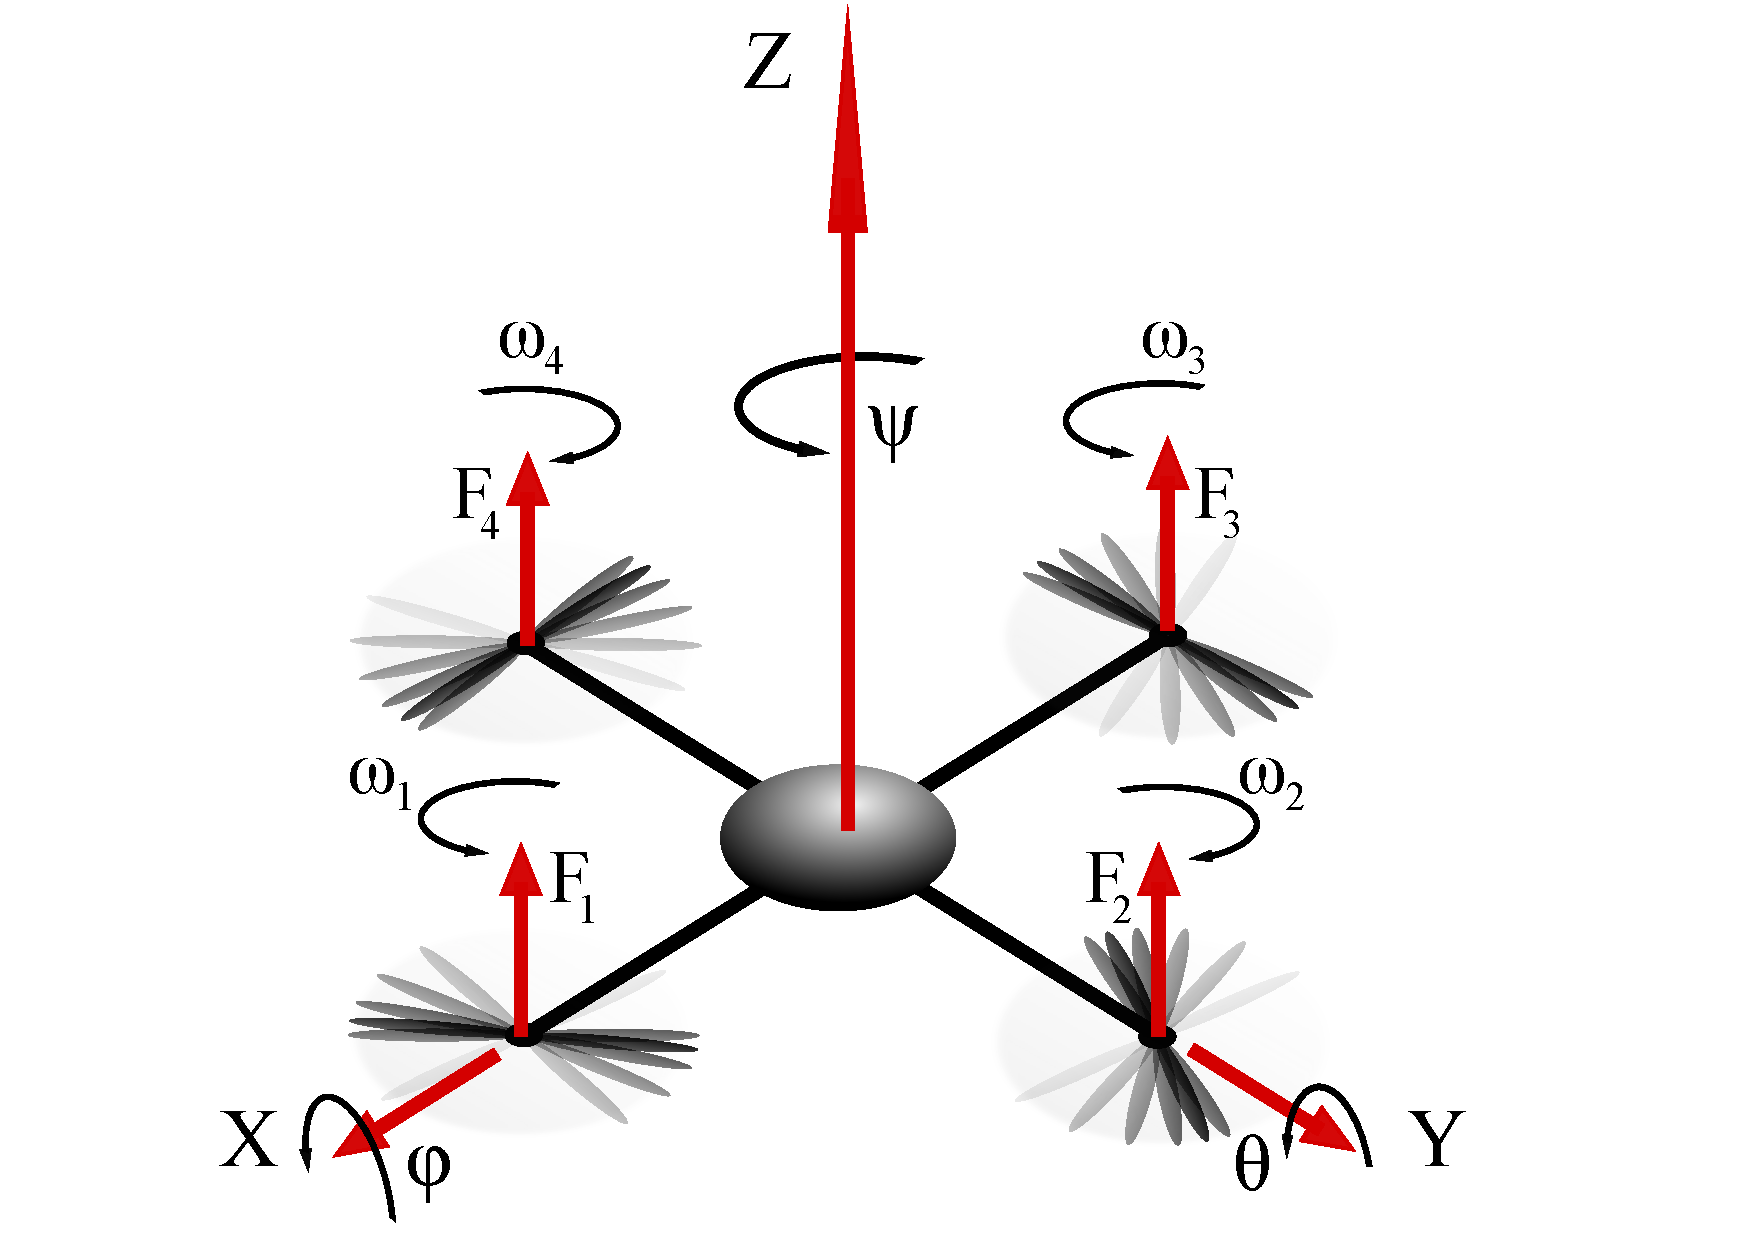
\includegraphics[width=0.8\textwidth]{images/Kraefte.pdf}
			\label{fig:Kraefte}
		\end{figure}
	\end{frame}

	\begin{frame}
		\frametitle{Newton-Euler Equations}
			\begin{columns}[T] % align columns
				\begin{column}{0.70\textwidth}
					Forces \\
					\[ F_{ext} = F_{g} + \sum_{i=1}^{4}{F_{i}} \]
					Torques \\
					\[ \tau_{ext} = \sum_{i=1}^{4}{\tau_{i}}+(\tau_{\varphi}+\tau_{\theta}) \]
				\end{column}
			\hfill
			\begin{column}{.25\textwidth}
				\begin{textblock}{0}(-2,1)
					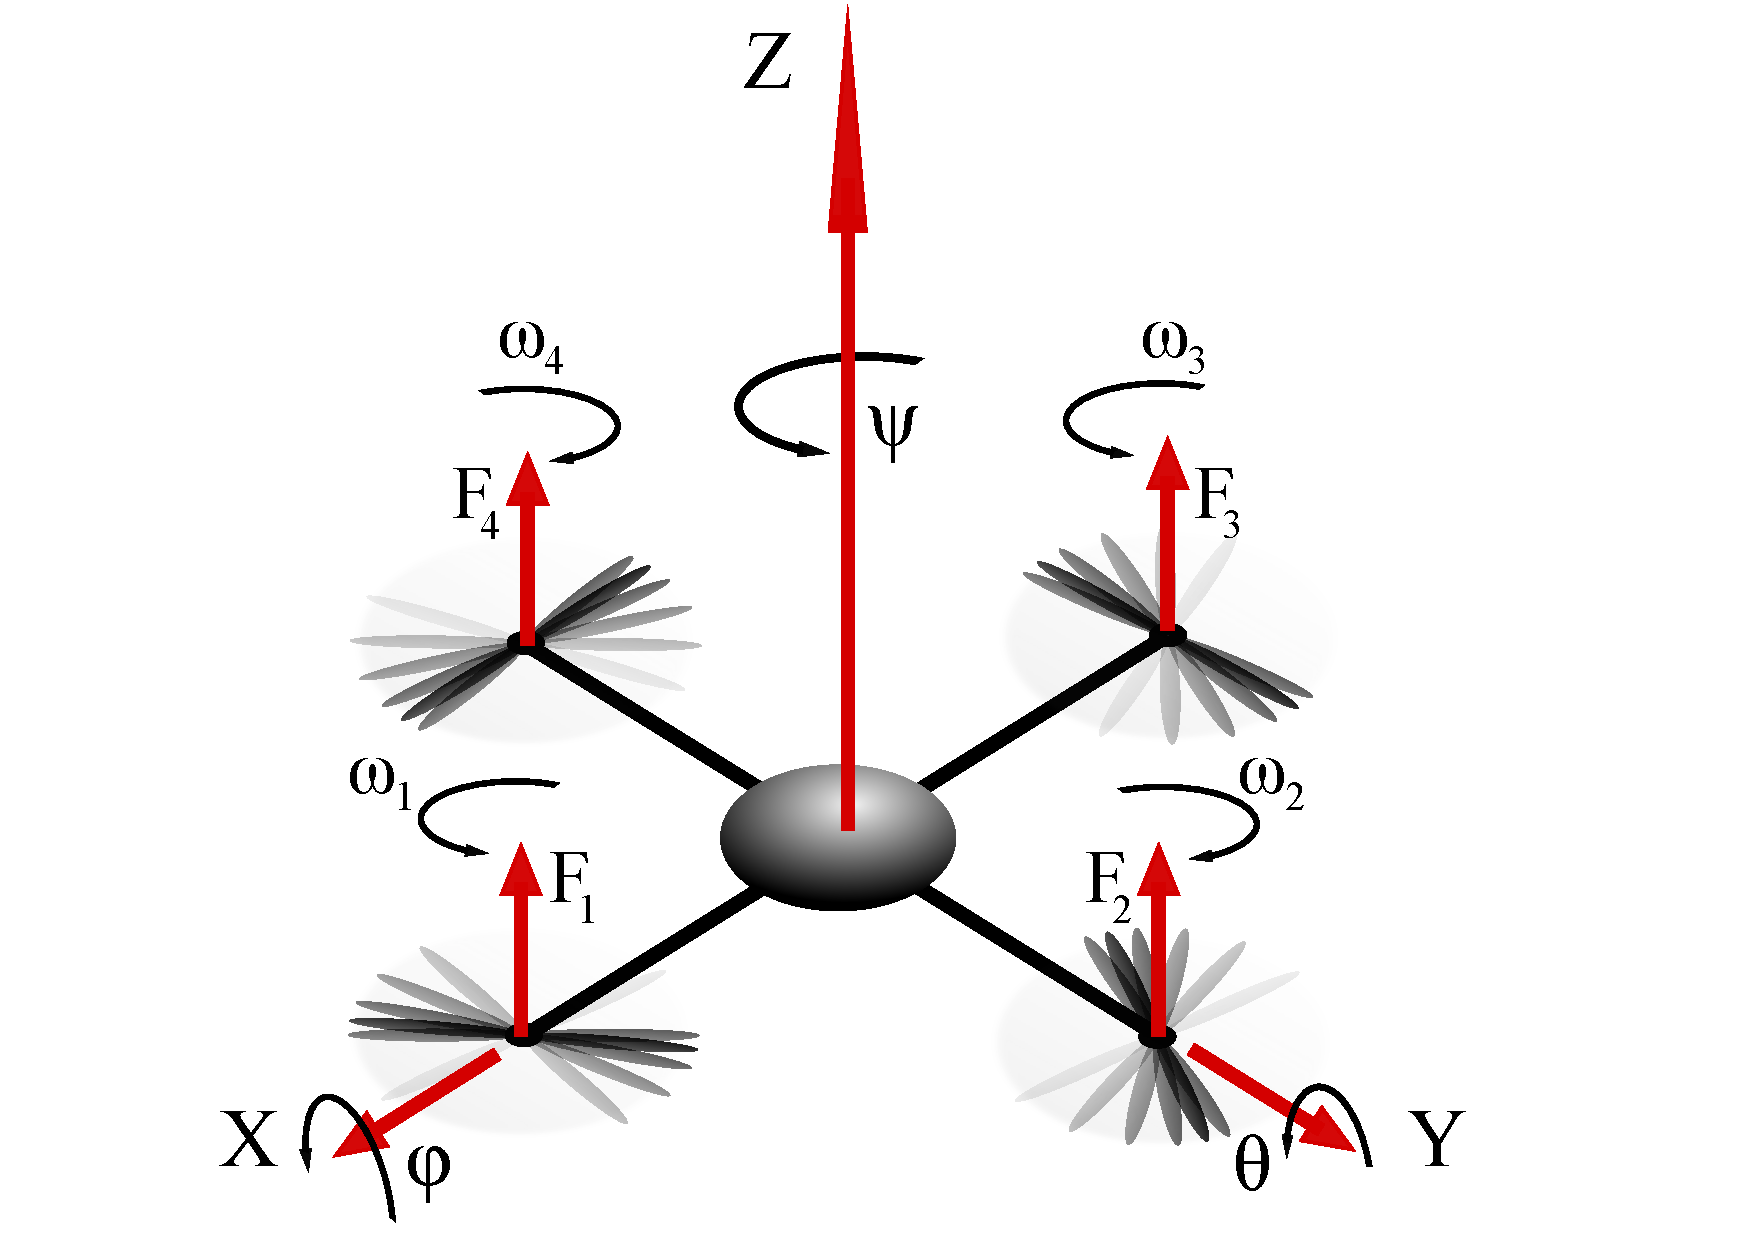
\includegraphics[width=5cm]{images/Kraefte.pdf}
					\label{fig:Kraefte klein}
				\end{textblock}
			\end{column}
		\end{columns}
	\end{frame}
		
	\begin{frame}
		\section{Model}
		\frametitle{Coordinate Systems}
			\begin{figure}[p]
				\centering
				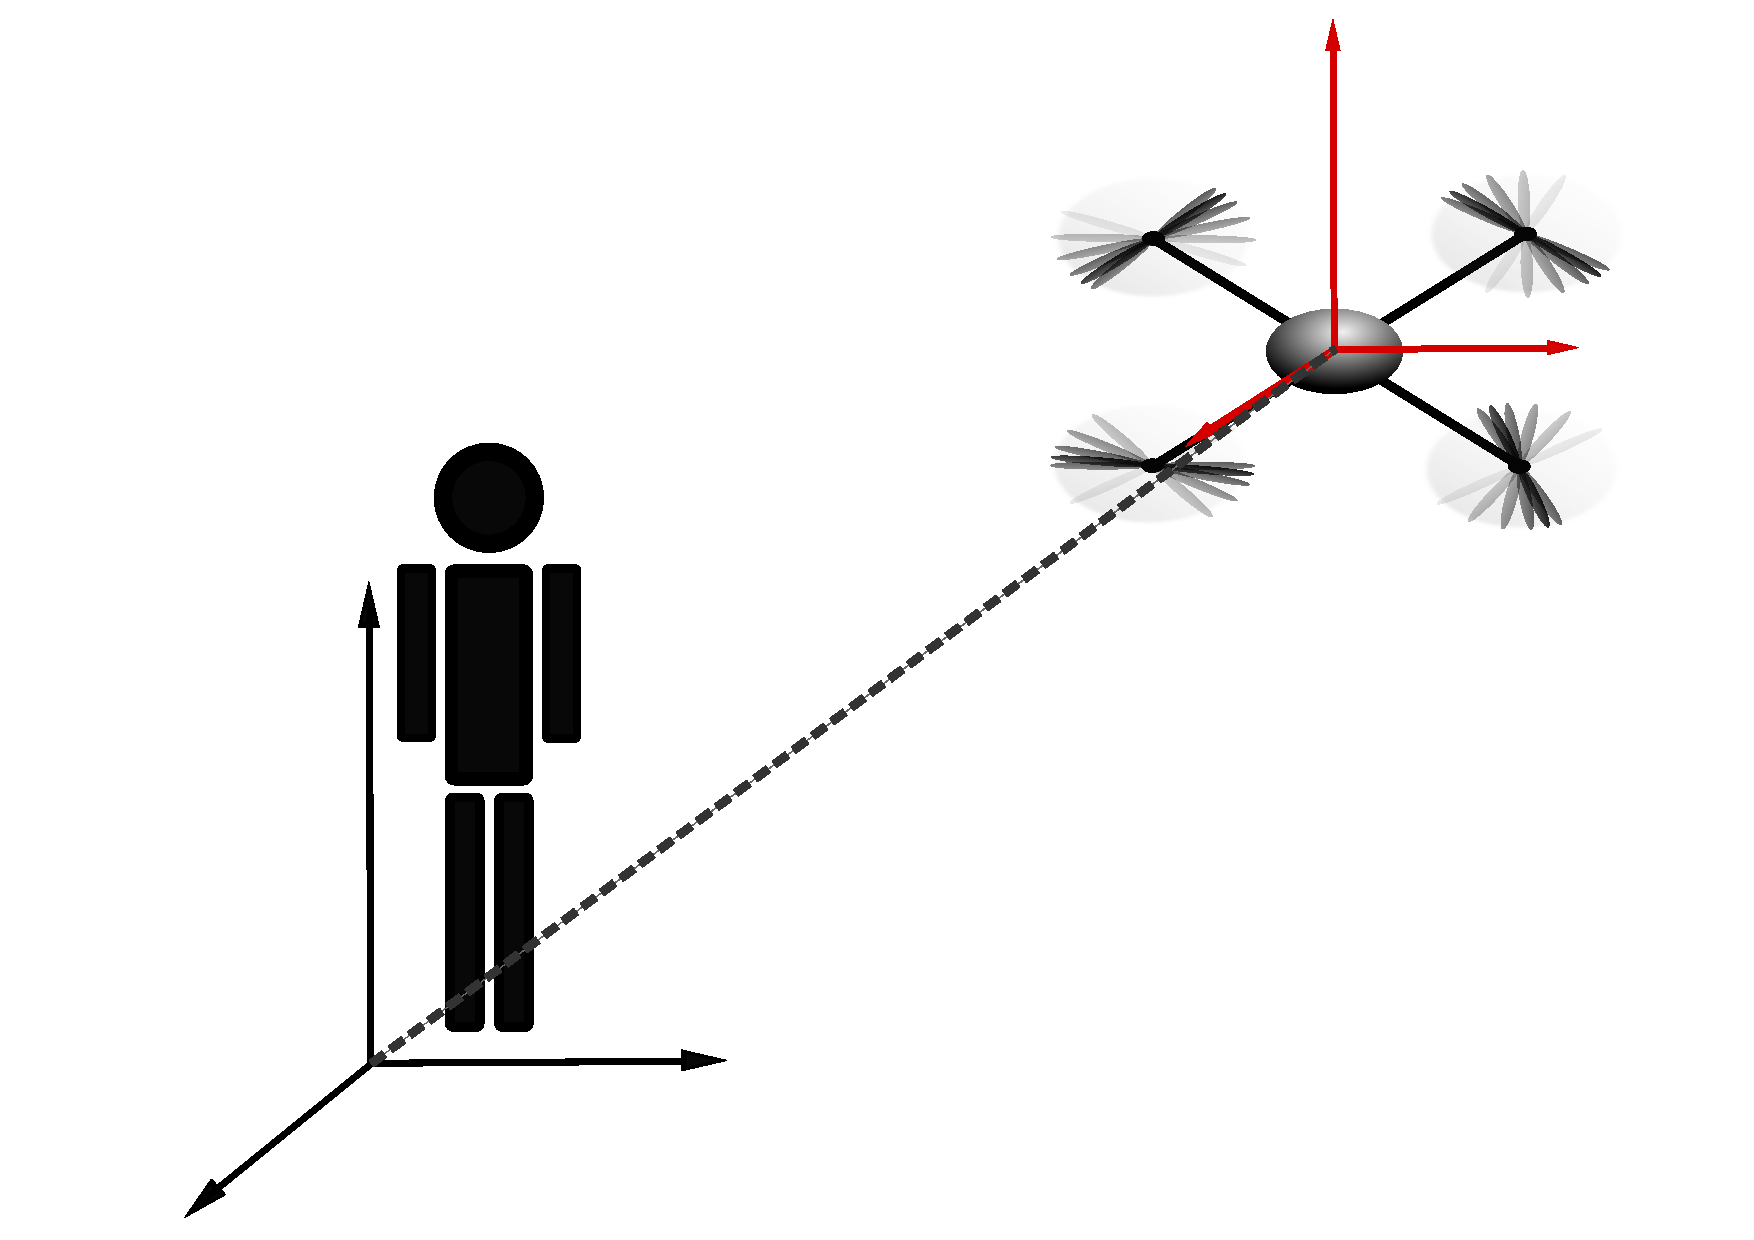
\includegraphics[width=0.8\textwidth]{images/Koordinatensysteme.pdf}
				\label{fig:Koordinatensysteme}
		\end{figure}
	\end{frame}

	
	\begin{frame}
		\frametitle{Quaternions}
		\begin{block}{}
			\[ q = a + \textup{i}b+\textup{j}c+\textup{k}d \qquad a, b, c, d \in \mathbb{R} \]
			\vspace{.1ex}
			\end{block}
			
			\vspace{1ex}
			\onslide<2-> representing rotation \( \Leftrightarrow \) \( \Vert q \Vert = 1 \) \\
			\vspace{1ex}			
			\onslide<3-> advantage \(\rightarrow\) no singularities \\
			\vspace{1ex}
			\onslide<4-> problem \(\rightarrow\) \( \Vert q \Vert = 1 \) additional constraint
	\end{frame}
	
	\begin{frame}
		\frametitle{Dynamics}
		Equations representing dynamics...
		\[ T(x, u) = M \cdot \begin{pmatrix} \dot{x}_{8} \\ \vdots \\ \dot{x}_{13} \end{pmatrix} + \Theta(x) \]
		\onslide<2->
		...expressed as system of differential equations:
		\[ \frac{\textup{d}}{\textup{d}t} 
			\begin{pmatrix}
						  x_{1} \\ \vdots \\ x_{7} \\ x_{8} \\ \vdots \\ x_{13}
			\end{pmatrix}
			=
			\begin{pmatrix}
							\dot{x}_{1} \\ \vdots \\ \dot{x}_{7} \\ M^{-1}(T(x,u)-\Theta(x))
			\end{pmatrix}
		\]
	\end{frame}
	
	\begin{frame}
		\frametitle{Prospect}
			Refinement of the model \\
			\vspace{1ex}
			\(\rightarrow\) wind \\
			\vspace{1ex}
			\(\rightarrow\) aerodynamical forces \\
	\end{frame}

%Der Befehl \include{datei} setzt dann hier die Datei datei.tex ,welche im selben Ordner liegt ein. Diese darf keinen Header enthalten
%\include{datei}
	\caption{Modell mit Warburg - Impedanz}
	\label{fig:WModell}
\end{figure}



